\documentclass[output=paper]{langscibook}
\author{Nina Radkevich\affiliation{University of York}}
\title{Backward vs. forward control/raising: A case of Lak aspectual verbs}
\abstract{This paper presents novel data from Lak exemplifying morpho-syntactic properties of aspectual verbs ‘to begin’ and ‘to finish’. The aspectual verbs in Tsez \citep{PolinskyPotsdam2002}, a language related to Lak, have been analysed as either backward control or raising depending on a number of their syntactic characteristics. When applied to Lak, the same tests produce a different result - the Lak aspectual verbs do not pattern with either control or raising. It is suggested that the aspectual construction is an example of clause union. The evidence in support of this proposal comes from A'-movement, agreement, and transitivity harmony.}
  
\begin{document}
\SetupAffiliations{mark style=none}
\maketitle

\section{Introduction}
The phenomenon of control and raising has been one of the most discussed topics in syntax \citep{hornstein1999,Landau2001,Landau2003,Landau2004,martin2001,BoeckxHornstein2003,BoeckxHornstein2004,DaviesDubinsky2004,Wurmbrand1999,wurmbrand2001,Wurmbrand2007} covering such issues as the nature of null elements (PRO, copies, traces, etc.) and complement sizes.\footnote{The list of references is not intended to be exhaustive but for the reasons of space I have chosen just a small representative subset of the literature on control and raising.} The recent shift of attention to a more cross-linguistic perspective  has enriched the typology of attested types of control and raising constructions providing us with a better understanding of their syntactic and semantic properties. One such discovery started with a seminal work by \citet{PolinskyPotsdam2002} which reported a previously unattested “backward control” construction from Tsez, Nakh-Dagestanian, as in (\ref{Rad1}) where the subject bears the case determined in the embedded clause. \citet{PolinskyPotsdam2002} analyse the construction in (\ref{Rad1}) as an instance of backward control, as schematically shown in (\ref{Rad2}). Interestingly, backward raising is also attested cross-linguistically, e.g., in Adyghe, North West Caucasian \citep{PotsdamPolinsky2012}.  
\ea\label{Rad1}
\gll Kid-bā ziya b-išr-a y-oq-si. \\
girl.\textsc{ii-erg} 		cow\textsc{.iii.sg.abs} 	\textsc{iii.sg}-feed-\textsc{inf} \textsc{ii.sg}-begin-\textsc{pst.evid}\\
\glt ‘The girl began to feed the cow.’    \citep[248]{PolinskyPotsdam2002}
\z 

\ea\label{Rad2}
$[$PRO\textsubscript{ABS}  $[$\textsubscript{XP} DP\textsubscript{ERG}  (DP\textsubscript{ABS})  V\textsubscript{INF}$]$  begin$]$\\
\z


In this paper, I will discuss one construction found in Lak,\footnote{All the Lak data in the paper are from author's fieldnotes.} a language related to Tsez, where the subject of the main clause has its case determined by the embedded verb, as in (\ref{Rad3}).\footnote{I use the < > notation in glosses to indicate that class agreement is realized as an infix.} 

\ea\label{Rad3}
\gll Rasul-lu-l lu 	buwk:un-nu q:urtal b-un-ni.\\
Rasul-\textsc{os-erg} 		book.\textsc{iii.sg.abs} 	\textsc{$<$iii.sg$>$}read-\textsc{prf.ger}	finish 		\textsc{iii.sg}-do-\textsc{pst.3}\\
\glt ‘Rasul finished reading a/the book.’
\z
Despite some surface similarities between the two constructions in Lak and Tsez, I will show that in Lak we deal with a mono-clausal structure. Capitalizing on the seminal work by \citet{wurmbrand2001,Wurmbrand2004,Wurmbrand2007}, I will argue that the aspectual verbs (‘to begin’ and ‘to finish) in Lak are restructuring verbs that can take complements of a much smaller size than CP/IP (cf. their Tsez counterparts).
The paper is organized as follows. First, I present a short sketch of Lak morpho-syntax to help the reader navigate through the data presented in the paper. In the next section, I introduce the key properties of the aspectual verb construction and compare its properties to the Tsez backward cases. Then, I will present additional data from Lak that has to do with so-called “transitivity concord/agreement” attested in various languages of the world \citep{Zariquiey2014}. The phenomenon of “transitivity agreement” observed in the Lak aspectual verb construction provides further evidence for its mono-clausal nature. Finally, I summarize the findings of the paper and identify directions for future research.

\section{Basics of Lak morpho-syntax}\label{Radsect2}
Lak is a Nakh-Dagestanian (or North East Caucasian) language spoken in the Republic of Dagestan in Russia. According to the 2010 census of the Russian Federation, there are 145,895 speakers. Lak forms its own branch of the Nakh-Dagestanian language family but shares many key morpho-syntactic properties with other members of the family previously studied formally: Tsez (Tsezic branch) and Archi (Lezgic branch). For more detailed descriptions of Lak morphosyntax discussed in this section, I refer the reader to  grammars of Lak (\citealt{Zhirkov1955}, \citealt{Murkelinskij1971}) and a comprehensive overview of Lak syntax in \citet{Kazenin2013}.

One of the most prominent features of Nakh-Dagestanian is its nominal class system: all nouns belong to one of the classes. The nominal class system is only partially determined by semantics (for humans). Importantly, the class is not overtly marked on nouns themselves but is revealed via agreement on other verbal and non-verbal elements of the clause. The number of classes across the family varies from 0 (Lezgian \citep{Haspelmath1993}, Aghul \citep{Magometov1970}, Udi \citep{Harris2002}, some dialects of Tabasaran \citep{Magometov1965}) to 8 (Batsbi \citep{Desheriev1967}). Lak has a system of four nominal classes where Class I is comprised of male human individuals, Class II is used for older females, Class III consists of nouns referring to females, animates, concrete and abstract concepts, and Class IV is made up of most abstract and some concrete nouns.

Furthermore, Lak has a rich system of case marking which can be split into two: core and spatial cases, with the latter being an instance of PPs (see \citet{Radkevich2010} for more detail and discussion). As for the core cases, Lak has absolutive, ergative, genitive, and dative cases. Some clarifications are in order here: 1) as common for Nakh-Dagestanian, absolutive is unmarked; 2) genitive and ergative are syncretic for nouns but not for pronouns; 3) non-absolutive forms of nouns usually have an additional morpheme between the root and the case exponent which is called an ‘oblique stem marker’.
Similarly to other members of the family, Lak is a head final morphologically ergative language where arguments of all intransitive verbs pattern with internal arguments of transitive verbs with respect to case marking, i.e., absolutive, whereas external arguments of transitive verbs\footnote{In this paper I will use the term 'external argument' to refer to external arguments of transitive verbs only excluding external arguments of unergative verbs.} can be either ergative or dative. Consider the following examples.

\ea\label{Rad6}
\gll Ninu d-urkun-ni.\\
mother.\textsc{ii.sg.abs} \textsc{ii.sg}-\textsc{<ii.sg>}come.\textsc{prf}-\textsc{pst.3}\\
\glt ‘Mother came.’
\z

\ea\label{Rad7}
\gll Ninu d-i:zun-ni.\\
mother.\textsc{ii.sg.abs} \textsc{ii.sg}-get.up-\textsc{pst.3}\\
\glt ‘Mother got up.’
\z

\ea\label{Rad8}
\gll Rasul-lu-l q:u dirχ:un-ni.\\
Rasul-\textsc{os-erg} field.\textsc{iv.sg.abs} \textsc{<iv.sg>}dig.\textsc{prf-pst.3}\\
\glt ‘Rasul dug up the field.’
\z

\ea\label{Rad9}
\gll T:u-n ga k:awk:un-ni.\\ 
\textsc{1.sg.iii-dat} he.\textsc{i.sg.abs} \textsc{<i.sg>}see.\textsc{prf-pst.3}\\
\glt ‘I saw him.’
\z

In (\ref{Rad6}) and (\ref{Rad7}), the sole arguments of intransitive verbs are absolutive marked. 
The situation is different in transitive clauses: 
in (\ref{Rad8}) and (\ref{Rad9}), the internal arguments are absolutive, while the external ones are ergative and dative, respectively. 
Another important property of Lak is absolutive controlled agreement: agreement can only be controlled by absolutive marked arguments. 
Most Nakh-Dagestanian languages have class/number agreement which is also true for Lak: 
class/number agreement is realized as prefixes, if vowel initial, as in (\ref{Rad6}-\ref{Rad7}), 
and/or infixes in the perfective aspect, as in (\ref{Rad6}), (\ref{Rad8}), and (\ref{Rad9}). 
This type of agreement is encoded with Roman numerals in the glosses. 
Furthermore, Lak has developed a person agreement system found on finite verbs: 
this type of agreement is also controlled by absolutive arguments and is realized as suffixes (glossed with Arabic numerals), as illustrated below.

\ea\label{Rad10}
\gll Na zu b-uwhunu b-ur-u.\\
\textsc{1.i.sg}  \textsc{2.i.pl} \textsc{i.pl-$<$i.pl$>$}catch.\textsc{prf.ger} \textsc{i.pl-aux-1/2pl}\\
\glt ‘I caught you.’
\z

\ea\label{Rad11}
\gll Na ga $∅$-uwhunu $∅$-ur-$∅$.\\
\textsc{1.i.sg}	\textsc{3.i.sg.abs} \textsc{i.sg-$<$i.pl$>$}catch.\textsc{prf.ger} \textsc{i.sg-aux-3}\\
\glt ‘I caught him.’
\z
Furthermore, Lak has contexts where the regular ergative-absolutive alignment in transitive clauses breaks down, i.e., the so-called cases of split ergativity. Lak has two types of split ergativity: aspect and person/tense based. In this description of Lak morpho-syntax, I will focus only on the former as the person/tense split ergativity is a very complicated phenomenon and is not directly relevant to the issue under discussion.

The aspect based split ergativity arises in imperfective durative (progressive) forms. External arguments of agentive verbs do not get their expected ergative marking, instead they appear absolutive marked. Furthermore, there are two agreement controllers where the internal argument controls class/number agreement on the lexical verb, while the absolutive marked external argument controls class/number and person agreement on the auxiliary verbs. Consider the examples in (\ref{Rad12}) and (\ref{Rad13}).

\ea\label{Rad12}
\gll Rasul č:itu b-uh-laj $∅$-ur-$∅$.\\
Rasul.\textsc{i.sg} cat.\textsc{iii.sg.abs} \textsc{iii.sg.abs}-catch-\textsc{dur.ger} \textsc{i.sg-aux-3}\\
\glt ‘Rasul is catching a/the cat.’
\z

\ea\label{Rad13}
\gll Rasul-lu-l č:itu b-uwhunu b-ur-$∅$.\\
Rasul.\textsc{i.sg-os-erg} cat.\textsc{iii.sg.abs} \textsc{iii.sg-$<$iii.sg$>$}catch.\textsc{prf.ger} \textsc{iii.sg-aux-3}\\
\glt ‘Rasul caught a/the cat.’
\z

In (\ref{Rad12}), the verb ‘to catch’ is used in the progressive aspect and its external argument ‘Rasul’ is absolutive marked, whereas it is ergative in non-progressive contexts, as in (\ref{Rad13}). Furthermore, the lexical verb agrees in class/number with the internal argument ‘cat’, whereas the auxiliary verb agrees with the absolutive marked external argument. In (\ref{Rad13}), however, all agreement is controlled by the internal argument \textit{č:itu} ‘cat’. Importantly, the aspect based split ergativity does not affect the so-called dative verbs, as in (\ref{Rad14}).\footnote{There are many other intricate properties of the Lak aspect based split ergativity but their discussion goes beyond the scope of the paper. For more detailed discussion and analysis I refer the reader to \citet{GagliardiRadkevich2014}.} 

\ea\label{Rad14}
\ea[]{
\gll Rasul-lu-n 	matematika q:a-d-urč’laj d-ur-$∅$.\\	  
Rasul.\textsc{i.sg-os-dat}  math.\textsc{iv.sg.abs} \textsc{neg-iv.sg}-understand.\textsc{dur.ger} 	\textsc{iv.sg-aux-3}\\
\glt 'Rasul does not understand math.'
}

\ex[*]{
\gll Rasul 	matematika q:a-d-urč’laj $∅$-ur-$∅$.\\	  
Rasul  math.\textsc{iv.sg.abs} \textsc{neg-iv.sg}-understand.\textsc{dur.ger} 	\textsc{iv.sg-aux-3}\\
}
\z
\z

The final aspect of Lak morpho-syntax that is directly relevant for this paper is word order and A'-movement. Like many other Nakh-Dagestanian languages, Lak has a relatively free word order within the clause, as illustrated below.

\ea\label{Rad15}
\ea{
\gll Rasul-lu-l q:u dirχ:un-ni.\\
Rasul.\textsc{i.sg-os-erg} field.\textsc{iv.sg.abs} \textsc{$<$iv.sg$>$}dig.\textsc{prf-pst.3}\\
\glt ‘Rasul dug up the field.’
}

\ex{
q:u Rasul-lu-l dirχ:un-ni.\\
}

\ex{
Rasul-lu-l dirχ:un-ni q:u.\\
}

\ex{
dirχ:un-ni Rasul-lu-l q:u.\\
}
\z
\z

However, long-distance scrambling is impossible, as shown in (\ref{Rad16}).

\ea\label{Rad16}
\ea[]{
\gll Rasul-lu-l buwsun-ni	$[$A\textsuperscript{ʕ}li-l pu\textsuperscript{ʕ}run ɣawɣ-šiwu$]$.\\
Rasul.\textsc{i.sg-os-erg} \textsc{$<$iii.sg$>$}say.\textsc{prf-pst.3} Ali.\textsc{i.sg-erg} glass.\textsc{iv.sg.abs} \textsc{<iv.sg>}break.\textsc{prf-msd}\\
\glt ‘Rasul said that Ali broke the window.’
 }

\ex[*]{
\gll Rasul-l-ul pu\textsuperscript{ʕ}run\textsubscript{i}	buwsun-ni, $[$A\textsuperscript{ʕ}li-l t\textsubscript{i} ɣawɣ-šiwu$]$.\\
Rasul.\textsc{i.sg-os-erg} glass.\textsc{iv.sg.abs} \textsc{$<$iii.sg$>$}say.\textsc{prf-pst.3} Ali.\textsc{i.sg-erg} t \textsc{<iv.sg>}break.\textsc{prf-msd}\\ 
}

\ex[*]{
\gll Pu\textsuperscript{ʕ}run\textsubscript{i} Rasul-lu-l buwsun-ni	$[$A\textsuperscript{ʕ}li-l  t\textsubscript{i} ɣawɣ-šiwu$]$.\\
glass.\textsc{iv.sg.abs} Rasul.\textsc{i.sg-os-erg} \textsc{$<$iii.sg$>$}say.\textsc{prf-pst.3} Ali.\textsc{i.sg-erg} t \textsc{<iv.sg>}break.\textsc{prf-msd}\\
 }	    													
\z 
\z

Furthermore, the same locality restrictions are found in wh-questions: namely, wh-word can optionally front to the sentence initial position, as in (\ref{Rad17}),  but it cannot cross the clausal boundary, as in (\ref{Rad18}).

\ea\label{Rad17}
\ea{
\gll Rasul-lu-l ci dirχ:un-ni?\\
Rasul-\textsc{os-erg} what.\textsc{iv.sg.abs} \textsc{$<$iv.sg$>$}dig.\textsc{prf-pst.3}\\
\glt ‘What did Rasul dig?’
}
\ex{
\gll Ci Rasul-lu-l dirχ:un-ni?\\
 what.\textsc{iv.sg.abs} Rasul-\textsc{os-erg}		 				\textsc{$<$iv.sg$>$}dig.\textsc{prf-pst.3}\\
}
\z
\z

\ea\label{Rad18}
\ea[]{
\gll Nit:i-n k’ul-s:a-r-iw, $[$Rasul	ci	d-ullaj-s:a-r-iw$]$?\\		
mother-\textsc{dat} 	know-\textsc{part-pres.3-q} Rasul.\textsc{i.sg.abs}	what.\textsc{iv.sg.abs} \textsc{iv.sg}-do.\textsc{dur.ger-part-pres.3-q}\\
\glt 'Does mother know what Rasul is doing?'
}

\ex[*]{
\gll Ci\textsubscript{i} nit:i-n k’ul-s:a-r-iw, $[$Rasul t\textsubscript{i}	d-ullaj-s:a-r-iw$]$?\\		
what.\textsc{iv.sg.abs} mother-\textsc{dat} 	know-\textsc{part-pres.3-q} Rasul.\textsc{i.sg.abs}	t \textsc{iv.sg}-do.\textsc{dur.ger-part-pres.3-q}\\
}


\ex[*]{
\gll Nit:i-n ci\textsubscript{i} k’ul-s:a-r-iw, $[$Rasul t\textsubscript{i}	d-ullaj-s:a-r-iw$]$?\\
mother-\textsc{dat} what.\textsc{iv.sg.abs}	know-\textsc{part-pres.3-q} Rasul.\textsc{i.sg.abs}	t \textsc{iv.sg}-do.\textsc{dur.ger-part-pres.3-q}\\
}
\z
\z

Having discussed the key properties of Lak morpho-syntax, in the next section I will present data from the aspectual verb construction and compare it to its Tsez counterpart highlighting many differences between the superficially similar constructions in the two languages.\\

\section{Aspectual verbs in Lak and Tsez}\label{Radsect:3}
In their seminal work, \citet{PolinskyPotsdam2002} study two interesting constructions with aspectual verbs in Tsez to conclude that one of them involves the so-called backward control, while the other is an instance of raising. The two structures in question are in (\ref{Rad19}) and (\ref{Rad20}). 

\ea\label{Rad19}
\gll Kid-bā 	ziya b-išr-a y-oq-si.\\
girl.\textsc{ii-erg} cow.\textsc{iii.abs} \textsc{iii}-feed-\textsc{inf} \textsc{ii}-begin-\textsc{pst.evid}\\
\glt ‘The girl began to feed the cow.’
\z

\ea\label{Rad20}
\gll Kid 	ziya b-išr-a y-oq-si.\\
girl.\textsc{ii.abs} cow.\textsc{iii.abs} \textsc{iii}-feed-\textsc{inf} \textsc{ii}-begin-\textsc{pst.evid}\\
\glt ‘The girl began to feed the cow.’ (\citealt[248-249]{PolinskyPotsdam2002})
\z

There are two surface differences between the two sentences that have to do with case marking and agreement: 1) in (\ref{Rad19}) the DP ‘girl’ bears ergative case associated with the embedded verb, while in (\ref{Rad20}) the same DP is absolutive marked; 2) the agreement on the main verb ‘to begin’  is controlled by the ergative DP, which is unattested in Tsez and in other Nakh-Dagestanian languages, whereas in the second sentence the controller is the absolutive DP ‘girl’. \citet{PolinskyPotsdam2002} propose that the two sentences under discussion have two different structures and, thus, represent different phenomena (control vs. raising). 

\ea\label{Rad21}
$[$PRO $[$DP\textsubscript{ERG} DP\textsubscript{ABS} V\textsubscript{INF}$]$ begin$]$ (=(\ref{Rad19}))
\z

\ea\label{Rad22}
$[$DP\textsubscript{ABS} $[$t DP\textsubscript{ABS} V\textsubscript{INF}$]$ begin$]$ (=(\ref{Rad20}))
\z

The structure in (\ref{Rad21}) is a schematic representation of backward control where the null element (PRO) is in the main clause rather than in the embedded one as it would be in the run of the mill cases of forward control.\footnote{It is important to point out that \citet{PolinskyPotsdam2002} treat control as movement \citep{hornstein1999} and the ergative DP is an instance of the pronunciation of the lower copy.} \citet{PolinskyPotsdam2002} draw this conclusion based on a number of tests that contrast the two constructions. Interestingly, the verbs that can have backward control in Tsez are so-called aspectual verbs ‘to begin’, ‘to continue’, and ‘to stop/finish’. The Lak aspectual verbs ‘to begin’ and ‘to finish’ also show unexpected patterns of case marking: they can only bear the case assigned by the embedded verb.\footnote{Unlike Tsez, Lak does not have a verb ‘to continue’: its meaning is realized via aspectual marking.} In the rest of the chapter, I will discuss some properties of the Lak aspectual verbs with special attention to case distribution and then I apply the tests used for Tsez in \citet{PolinskyPotsdam2002} to the Lak aspectual verbs to show that Lak aspectual verbs do not fit the patterns displayed by their Tsez counterparts.\\

\subsection{Case distribution in the Lak aspectual construction}

The two Lak aspectual verbs (‘to begin’ and ‘to finish’) share a lot of similarities with respect to the distribution of case. The two aspectual verbs take gerunds as their complements: the verb ‘to begin’ takes gerunds in imperfective aspects, whereas the verb ‘to finish’ takes perfective gerunds. Furthermore, they behave identically with respect to case distribution when used without gerundial complements. Consider the following sentences illustrating case marking for the verb ‘to begin’.

\ea\label{Rad23}
\gll Bawa-l cila žahil-nij-s:a χawar b-ajbiwxun-ni.\\ 
grandmother.\textsc{ii-erg} self.\textsc{ii.sg} youth.\textsc{iv-loc-attr} story.\textsc{iii.sg.abs} 
\textsc{iii.sg-$<$iii.sg$>$}begin.\textsc{prf-pst.3}\\
\glt ‘Grandmother began her story about her youth.’
\z

The same pattern of case distribution holds for the verb ‘to finish’ as well. Consider the data below. In (\ref{Rad26}), similarly to (\ref{Rad23}), the external argument is ergative.

\ea\label{Rad26}
\gll Bawa-l cila žahil-nij-s:a χawar q:urtal b-un-ni.\\ 	
grandmother.\textsc{ii-erg} self.\textsc{ii.sg} youth.\textsc{iv-loc-attr} story.\textsc{iii.sg.abs}	finish \textsc{iii.sg}-do-\textsc{pst.3}\\ 
\glt ‘Grandmother finished her story about her youth.’
\z

Whenever the verb ‘to begin’ is used on its own, i.e., without an embedded verb, (\ref{Rad23}), its external argument is ergative but when it is used with the gerundial complement in (\ref{Rad24}), the external argument of the embedded verb \textit{bawa} ‘grandmother’ is absolutive marked. This case marking is compatible with the Lak case marking in durative (imperfective) contexts, i.e., split-ergativity. Note that the main verb is in the perfective aspect which is impossible with the absolutive marked external argument. Furthermore, if the embedded verb has a dative alignment, it is preserved in the aspectual construction. Given the data in (\ref{Rad23}-\ref{Rad25}), the case marking is determined in the embedded clause.

\ea\label{Rad24}
\gll Bawa o\textsuperscript{ʕ}l t:izlaj d-ajdirxun-ni.\\ 	
grandmother.\textsc{ii.sg.abs} cow.\textsc{iii.sg.abs} milk.\textsc{dur} \textsc{ii.sg-$<$ii.sg$>$}begin.\textsc{prf-pst.3}\\ 
\glt ‘Grandmother began milking a/the cow.’
\z



\ea\label{Rad25}

\gll A\textsuperscript{ʕ}li-n matematika d-urč’laj	d-ajdirxun-ni.\\
Ali-\textsc{dat} math.\textsc{iv.sg.abs} \textsc{iv.sg}-understand.\textsc{dur} \textsc{iv.sg-$<$iv.sg$>$}begin.\textsc{prf-pst.3}\\
\glt ‘Ali began to understand math.’
\z 


 Furthermore, the verb ‘to finish’ takes perfective gerunds as its complement and that aspect is incompatible with split ergativity, i.e., the external argument cannot be absolutive, as can be seen in (\ref{Rad27}). 
 \largerpage
 
\ea\label{Rad27}
\ea[] {
\gll A\textsuperscript{ʕ}jšat-lu-l huqa buruw:un-nu q:urtal 	b-un-ni.\\
Ajšat.\textsc{iii-os-erg} dress.\textsc{iii.sg.abs} \textsc{$<$iii.sg$>$}sew.\textsc{prf-prf.ger} 	finish \textsc{iii.sg}-do-\textsc{pst.3}\\
\glt 'Aishat finished sewing a/the dress.'
}

\ex[*]{
\gll A\textsuperscript{ʕ}jšat huqa buruw:un-nu q:urtal 	b-un-ni.\\
Ajšat.\textsc{iii.sg.abs} dress.\textsc{iii.sg.abs} \textsc{$<$iii.sg$>$}sew.\textsc{prf-prf.ger} 	finish \textsc{iii.sg}-do-\textsc{pst.3}\\
}
\z 
\z 

To show that it is indeed the embedded clause properties that determine case marking, we can have the main verb in the durative aspect where the split ergativity (absolutive marking on external arguments) arises. This configuration makes straightforward testable predictions: 1) if the case is determined in the embedded clause, the external argument will be in ergative; 2) if the case is determined in the matrix clause, the external argument will be absolutive. Now consider the example in (\ref{Rad28}): the external argument ‘Aishat’ is ergative marked, consequently, the case of the external argument originates in the embedded clause.

\ea\label{Rad28}
\gll A\textsuperscript{ʕ}jšat-lu-l huqa buruw:un-nu q:urtal b-awaj	b-ur-$∅$.\\
Ajšat.\textsc{iii-os-erg} dress.\textsc{iii.sg.abs} \textsc{$<$iii.sg$>$}sew.\textsc{prf-prf.ger} finish \textsc{iii.sg}-do.\textsc{iter.dur.ger} \textsc{iii.sg-aux-3}\\
\glt ‘Aishat is finishing sewing a/the dress.’
\z 

Having determined that the external argument in the aspectual constructions in Lak gets its case in the embedded clause, it is important to establish the position of this argument, i.e., whether it stays in the embedded clause or moves to the main clause.\\

\subsection{Position of the external argument}
\citet{PolinskyPotsdam2002} apply a number of tests to show that in the case the backward control construction the external argument stays in the embedded clause, whereas in the case of raising, it moves to the matrix clause. To determine this, they use the following tests: 1) A'-movement (scrambling and wh-movement); 2) event quantification; 3) second position validation clitic; 4) complement ellipsis. In this paper, I will use only the first two tests since Lak does not have any item similar to the Tsez second position validation clitic and the phenomenon of complement ellipsis gives rise to more complications, a proper discussion of which goes beyond the scope of the current paper.

\subsubsection{A'-movement in the Lak aspectual construction}\label{Radsect:3.2.1}
In Tsez and in Lak, A'-movement is clause-bound as discussed in Section \ref{Radsect2} (see examples in (\ref{Rad15}-\ref{Rad18}).  This locality restriction on movement allows us to test the position of arguments in the aspectual constructions and decide whether the structure is mono-clausal or bi-clausal. Consider the following two examples used as a base for applying the movement tests.

\ea\label{Rad29}
\gll A\textsuperscript{ʕ}li q:at:a b-ullaj $∅$-ajiwxun-ni.\\
Ali.\textsc{i.sg.abs} house.\textsc{iii.sg.abs} \textsc{iii.sg}-do.\textsc{dur.ger} \textsc{i.sg-$<$i.sg$>$}begin.\textsc{prf-pst.3}\\
\glt ‘Ali began building a/the house.’
\z 

\ea\label{Rad30}
\gll A\textsuperscript{ʕ}li-l lu buwk:un-nu q:urtal b-un-ni.\\
 Ali.\textsc{i-erg} book.\textsc{iii.sg.abs} \textsc{<iii.sg>}read.\textsc{prf.ger} finish \textsc{iii.sg}-do-\textsc{pst.3}\\
\glt ‘Ali finished reading a/the book.’
\z 

Interestingly, (\ref{Rad29}) and (\ref{Rad30}) allow any word order combinations, thus suggesting that the structure is actually mono-clausal, as shown in (\ref{Rad31}) and (\ref{Rad32}).\footnote{An anonymous reviewer raises a question of whether the following word order is possible, as in (\ref{Radi}). The ungrammaticality of (\ref{Radi}) is not surprising since the complex verb \textit{q:urtal ban} forms a morpho-phonological unit which cannot be split even in clearly mono-clausal structures, as in (\ref{Radii}).

\ea\label{Radi}
\gll *Lu b-un-ni A\textsuperscript{ʕ}li-l buwk:un-nu q:urtal.\\
book.\textsc{iii.sg.abs} \textsc{iii.sg}-do-\textsc{pst.3} Ali.\textsc{i-erg}  \textsc{<iii.sg>}read.\textsc{prf-prf.ger} finish\\
\z

\ea\label{Radii}
\gll *χawar q:urtal bawa-l b-un-ni.\\
story.\textsc{iii.sg.abs} finish grandmother.\textsc{ii-erg} 
\textsc{iii.sg}-do-\textsc{pst.3}\\
\glt ‘Grandmother began her story.’
\z
}
Since it is a mono-clausal structure, the discussion of the position of the external argument in terms of embedded/matrix clauses is inapplicable.

\ea\label{Rad31}
\ea{
Q:at:a A\textsuperscript{ʕ}li b-ullaj $∅$-ajiwxun-ni.
}

\ex{ 
A\textsuperscript{ʕ}li b-ullaj q:at:a	$∅$-ajiwxun-ni.
}

\ex{
A\textsuperscript{ʕ}li $∅$-ajiwxun-ni q:at:a b-ullaj.
}

\ex{
A\textsuperscript{ʕ}li $∅$-ajiwxun-ni b-ullaj q:at:a.
}
\z
\z 

\ea\label{Rad32}
\ea{
Lu A\textsuperscript{ʕ}li-l buwk:un-nu q:urtal b-un-ni.
}

\ex{
A\textsuperscript{ʕ}li-l buwk:un-nu lu q:urtal b-un-ni.
}

\ex{ A\textsuperscript{ʕ}li-l q:urtal b-un-ni lu buwk:un-nu.
}

\ex{
A\textsuperscript{ʕ}li-l q:urtal b-un-ni buwk:un-nu lu.
}
\z 
\z 


\largerpage[2]
In this section, I have shown that the aspectual construction is mono-clausal as it allows scrambling compatible with the mono-clausal structure.\footnote{In this paper I do not test wh-questions in the Lak aspectual construction as it requires a more detailed discussion which is impossible due to the space limits. Thus, I leave it for future research.}

\subsubsection{Event quantification}
\citet{PolinskyPotsdam2002} use an event quantification test to argue for the two structures (backward control and raising), namely, they show that a temporal adverbial can be interpreted as either modifying the matrix or the embedded verb. Interestingly, the two constructions with the linearly identical position of the adverb can have two distinct interpretations. Consider the following pair to illustrate this point.

\ea\label{Rad35}
\gll $[$kidbā uyrax āłiru ziya bišra$]$ yoqsi.\\
 girl.\textsc{erg} fourth time cow feed began\\
\glt ‘The girl began to feed the cow for the fourth time.’ (=4 feedings)\\
*‘The girl began for the fourth time to feed the cow.’ (=4 beginnings)
\z 

\ea\label{Rad36}
\gll kid uyrax āłiru ziya bišra yoqsi.\\
girl.\textsc{abs} fourth time cow feed began\\
\glt ‘The girl began to feed the cow for the fourth time.’ (=4 feedings)\\
‘The girl began for the fourth time to feed the cow.’ (=4 beginnings) (\citealt[255]{PolinskyPotsdam2002})
\z 

In (\ref{Rad35}) and (\ref{Rad36}), the adverbial is placed after the external arguments ‘girl’. If DP ‘girl’ is in the embedded clause, the adverbial is located there as well, thus it can only modify the embedded predicate. If the DP is in the matrix clause, the adverbial can modify either the matrix or the embedded verb. In (\ref{Rad35}), the only available interpretation is that ‛the girl fed the cow four times’, i.e. the adverbial modifies the embedded clause, while (\ref{Rad36}) is ambiguous between ‘the girl fed the cow four times’ and ‘the girl had four beginning of cow-feeding’, i.e., the adverb modifies the matrix verb. To see how the same test fares in the Lak aspectual construction consider the following examples.

\ea\label{Rad37}
\gll Amudada k’ilčin o\textsuperscript{ʕ}l t:izlaj d-ajdirxun-ni.\\
grandmother.\textsc{ii.sg.abs} twice cow.\textsc{iii.sg.abs} milk.\textsc{dur.ger} \textsc{ii.sg-<ii.sg>}begin.\textsc{prf-pst.3}\\
\glt ‘Amudada began milking the cow for the second time.’ (two beginnings, \#two milkings)\\
\z 

\newpage
\ea\label{Rad38}
\gll Bawa-l k’ilčin cila χawar b-uwsu-nu q:urtal b-unni.\\
grandma.\textsc{ii-erg} twice self.\textsc{ii.sg} story.\textsc{iii.sg.abs} \textsc{iii.sg-<iii.sg>}tell.\textsc{prf-prf.ger} finish 	\textsc{iii.sg}-do-\textsc{pst.3}\\
\glt ‘Grandmother finished telling her story twice.’(two finishings, \#two stories)\\
\z 

The data in (\ref{Rad37}) and (\ref{Rad38}) parallel the examples from Tsez in (\ref{Rad35}) and (\ref{Rad36}): the adverbial followsr the external argument.  Interestingly, both Lak sentences are unambiguous: they can only mean ‘two beginnings’ and ‘two finishings’, respectively. In other words, the adverbial cannot modify the embedded verb, thus indicating that the external argument is in the matrix clause. 

Having applied the test of the event quantification to the Lak aspectual verb construction, I conclude that the aspectual constructions are mono-clausal which further corroborates the results reported in Section \ref{Radsect:3.2.1}.

\subsection{Types of external arguments}
\citet{PolinskyPotsdam2002}  provide another piece of evidence for teasing the two constructions (control vs. raising) apart: the two types of verbs vary with respect to what types of external arguments they can have which is due to differences in their thematic structure. First, they note that only control predicates are compatible with such adverbs as ‘intentionally’, whereas raising verbs are only possible with adverbs like ‘accidentally’. When applied to the Lak aspectual verbs, a different picture emerges: both verbs are compatible with both types of adverbs.

\ea\label{Rad41}
\gll Rasul ma\textsuperscript{ʕ}žannugu ok:inu duklaj	$∅$-ajiwxun-ni.\\
Rasul.\textsc{i.sg.abs} on.purpose bad study.\textsc{dur.ger} \textsc{i.sg-<i.sg>}begin.\textsc{prf-pst.3}\\
\glt ‘Rasul on purpose began not to study well.’
\z 

\ea\label{Rad42}
\gll A\textsuperscript{ʕ}li cakunu $∅$-ajiwxun-ni q:at:a b-ullaj.\\
Ali.\textsc{i.sg.abs} unexpectedly \textsc{i.sg-<i.sg>}begin.\textsc{prf-pst.3} house.\textsc{iii.sg.abs} \textsc{iii.sg}-do.\textsc{dur.ger}\\
\glt ‘Ali unexpectedly began building the/a house.’
\z 


\ea\label{Rad43}
\gll A\textsuperscript{ʕ}jšat-lu-l huqa b-uruwχ:un-nu ma\textsuperscript{ʕ}žannugu/cakunu q:urtal b-un-ni.\\
Ajšat-\textsc{os-erg} 	dress.\textsc{iii.sg.abs} \textsc{iii.sg-<iii.sg>}sew.\textsc{prf-prf.ger} on.purpose/unexpectedly	finish 	\textsc{iii.sg}-do-\textsc{pst.3}\\	
\glt ‛Aishat finished sewing a/the dress.’
\z 
Furthermore, it is also shown in \citet{PolinskyPotsdam2002} that control verbs can have animate subjects, whereas raising verbs can only have inanimate subjects, as expected if they are only compatible with the adverbs like ‘accidental’. In Lak, however, both aspectual verbs are possible with inanimate subjects, as in (\ref{Rad44}) and (\ref{Rad45}).   

\ea\label{Rad44}
\gll Marχ:ala baws:u-nu q:urtal xun-ni.\\
snow.\textsc{iii.sg.abs} \textsc{<iii.sg>}melt.\textsc{prf-prf.ger} finish become-\textsc{pst.3}\\
\glt ‘Snow finished melting/Snow has melted.’
\z 

\ea\label{Rad45}
\gll Marχ:ala baslaj b-ajbiwxu-ni.\\
snow.\textsc{iii.sg.abs} melt.\textsc{dur.ger} \textsc{iii.sg-<iii.sg>}begin-\textsc{pst.3}\\
\glt ‘Snow started melting.’
\z 

Finally, based on \citet{Farkas1988}, \cite{PolinskyPotsdam2002} also argue that raising verbs cannot be used in imperatives. The Lak aspectual verbs can be used in the imperative construction, as shown below.
\ea\label{Rad46}
\gll $∅$-ajixu balaj t’ij!\\
\textsc{i.sg}-begin.\textsc{imper} song.\textsc{iii.sg.abs} say.\textsc{dur.ger}\\
\glt ‘Start singing!’
\z 

\ea\label{Rad47}
\gll Q:urtal d-u-wa t’aħni-k’ič’u šuʕršu-nu!\\
finish \textsc{iv.sg}-do-\textsc{pot2}	crockery.\textsc{iv.sg}	\textsc{<iv.sg>}wash.\textsc{prf-prf.ger}\\
\glt ‘Stop washing dishes!’
\z 

The data presented in this section show that the Lak aspectual verbs behave neither like control nor like raising verbs: on the one hand, the external arguments are in the matrix clause but inherit case from the embedded clause being compatible with the raising structure, while on the other hand, the aspectual verb are compatible with animate and inanimate subject, volitional and non-volitional adverbs, and can be used in imperatives. To accommodate all of these properties of the Lak aspectual verbs, I propose that these verbs form a complex predicate with their embedded verbs (something similar to the serial verb construction). Additional evidence to support this proposal comes from agreement and transitivity harmony.

\section{Analysis: aspectual verbs as restructuring}
In the previous section I have applied several tests to Lak that are used by \citet{PolinskyPotsdam2002} to show that the aspectual construction in Tsez can be analysed either as (backward) control or raising. Unlike Tsez, its Lak counterparts behave neither as control nor as raising. In this section, I propose that the Lak aspectual construction is a case of restructuring (clause union). I base my proposal on the following pieces of evidence. First, as shown in Section \ref{Radsect:3}, this construction behaves as a mono-clausal structure with respect to A'-movement: scrambling is freely available despite this phenomenon being clause bound in Lak. Second, the Lak aspectual construction differs from Tsez in another important characteristic, namely agreement, which I will discuss later in this section. The final piece of evidence comes from a phenomenon strongly resembling the so-called ‘transitivity harmony’.

Before discussing the analysis of the aspectual construction, it is important to spell out some underlying assumptions regarding case and agreement in Lak. Following \cite{GagliardiRadkevich2014}, \citet{Radkevich2017},  I assume that in regular (non-split ergative) contexts  case is determined within vP, whereas in the biabsolutive construction the case on the external argument is checked higher in the clause (AspP). Additionally, it is important to point out that when the Asp is specified for the [\textsc{imperf}] feature, it also has an EPP-type feature which triggers the external argument to move out of vP. I also adopt an approach against multiple probing, i.e., when the same DP is targeted by several heads for feature valuation, as in \citet{PolinskyChumakina2017}. \footnote{For independent motivations for this assumption see \cite{Rezac2003}, \cite{BakerWillie2010}.} Furthermore, I follow an analysis to agreement proposed in \citet{PolinskyChumakina2017} where each verbal head in the clause bears unvalued [u\textsc{cl}] features which can be valued by the closest absolutive marked DP. Furthermore, \citet{PolinskyChumakina2017} propose a system where only the lowest verbal head gets its features valued by the absolutive DP, whereas [u\textsc{cl}] features on all other heads are valued by the closest v, as schematically illustrated in (\ref{Rad54}) (for similar proposals see \citealt{Collins2003}, \citealt{BakerWillie2010}): v2 gets its features checked by DP2, i.e., the closest absolutive DP, then v2 values the unvalued class/number features of v1 which in its turn values the same features on Asp. Importantly, I assume that feature valuation proceeds only in one direction -downward.


\ea\label{Rad54}

[\textsubscript{AspP} [\textsubscript{Asp$'$}[\textsubscript{vP2} DP1 [\textsubscript{v$'$} [\textsubscript{vP1} [\textsubscript{v$'$} [\textsubscript{VP} DP2 V]  v1\textsubscript{[u\textsc{cl}]}] v2 \textsubscript{[u\textsc{cl}]}] Asp\textsubscript{[u\textsc{cl}]}]]]]\\
\z

Going back to the aspectual construction in Lak, I propose that it should be analyzed as a case of restructuring as in (\ref{Rad48}).\footnote{Restructuring analyses of constructions resembling backward control have been proposed in \cite{Roussou2009} for Greek and in \cite{GreshlerWintner2017} for Modern Standard Arabic. I thank an anonymous review for pointing these references to me.} The aspectual verbs (vP) take a complement as large as AspP since the embedded verb is marked for aspect but smaller than CP and the external argument (DP1) undergoes movement from the embedded to the matrix clause:\footnote{An anonymous review has raised an interesting question of why DP1 does not get its case in the matrix clause. A possible solution is to assume that the original case of DP1 that it gets in the embedded clause cannot be overridden in the next cycle (matrix clause). Then, the next question is why DP1 moves to the matrix clause. I will leave this question for future research.}

\ea\label{Rad48}
[\textsubscript{vP} [\textsubscript{v$'$}[\textsubscript{AspP} [\textsubscript{Asp$'$}[\textsubscript{vP2} DP1 [\textsubscript{v$'$} [\textsubscript{vP1} [\textsubscript{v$'$} [\textsubscript{VP} DP2 V]  v1\textsubscript{[u\textsc{cl}]}] v2 \textsubscript{[u\textsc{cl}]}] Asp\textsubscript{[u\textsc{cl}]}] v\textsubscript{[u\textsc{cl}]}]]]]\\
\z 

The structure in (\ref{Rad48}) straightforwardly accounts for the agreement facts in the Lak aspectual constructions due to its mono-clausal status. Below I will illustrate how the proposal works with the two aspectual verbs. Consider the following derivation for the verb ‘to finish’ in (\ref{Rad55}), which is based on (\ref{Rad48}): the lowest v gets its [u\textsc{cl}] features valued by the absolutive DP (DP2), whereas the higher verbal elements get their values for [\textsc{cl}] from the closest verbal head.

\newpage
\ea\label{Rad55}	
Derivation for the verb 'to finish'
\hspace{-2em}
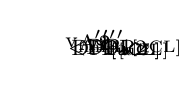
\begin{tikzpicture} \footnotesize
\Tree [.vP [.\node(x){DP1}; ] [.v$'$ [.AspP [.Spec ] [.Asp$'$ [.vP [.\node(y){$<$DP1$>$}; ] [.v$'$ [.vP [.Spec ] [.v$'$ [.VP [.\node(DP2){DP2}; ] [.V ] ] [.\node(v1){v1\textsubscript{[uCL]}}; ] ] ] [.\node(v2){v2\textsubscript{[uCL]}}; ] ] ] [.\node(Asp){Asp\textsubscript{[uCL]}}; ] ] ] [.\node(v){v\textsubscript{finish,[uCL]}}; ] ] ]

\draw [<-] (x) to [bend right=90] (y);
\draw [->] (v2) to [bend left=45] (v1);
\draw[->] (Asp) to [bend left=45] (v2);
\draw [->] (v) to [bend left=45] (Asp);
\draw[->] (v1) to [bend left=70] (DP2);
\end{tikzpicture}
\z 

The situation is slightly different for the verb ‘to begin’, (\ref{Rad56}): it has two absolutive arguments (=split ergativity) due to the aspectual specification of the embedded verb. In (\ref{Rad56}), v1 gets its [u\textsc{cl/num}] features valued by the closest absolutive marked DP, the internal argument, then v1 values features on v2, and v2 on Asp. Recall that in the system proposed in \citet{PolinskyChumakina2017}, agreement between heads applies as a last resort operation when there is no absolutive marked DP available for agreement. In (\ref{Rad56}), v\textsubscript{begin} has [u\textsc{cl}] features which are valued by the absolutive marked external argument (DP1).\footnote{The derivation for the verb ‘to begin’ is similar in spirit to the analysis of the biabsolutive construction in Lak \citep{Radkevich2017} and Archi \citep{Polinsky2016}. I refer the reader to these works for further discussion and detail.}

\newpage
\ea\label{Rad56}
Derivation for the verb 'to begin'\footnote{Recall that the verb 'to begin' takes imperfective gerundial complements which give rise to split ergativity. In the analysis of this phenomenon adopted in the paper, the external argument raises to spec,AspP in the split-ergative context. In the diagram in (\ref{Rad56}) I omit this part for the ease of exposition.} 

\begin{tikzpicture}
\footnotesize
\Tree [.vP [.\node(x){DP1}; ] [.v$'$ [.AspP [.Spec ] [.Asp$'$ [.vP [.\node(y){$<$DP1$>$}; ] [.v$'$ [.vP [.Spec ] [.v$'$ [.VP [.\node(DP2){DP2}; ] [.V ] ] [.\node(v1){v1\textsubscript{[uCL]}}; ] ] ] [.\node(v2){v2\textsubscript{[uCL]}}; ] ] ] [.\node(Asp){Asp\textsubscript{[uCL]}}; ] ] ] [.\node(v){v\textsubscript{begin [uCL]}}; ] ] ]

\draw [<-] (x) to [bend right=90] (y);
\draw [->] (v2) to [bend left=45] (v1);
\draw[->] (Asp) to [bend left=45] (v2);
\draw [->] (v) to [bend left=20] (x);
\draw[->] (v1) to [bend left=70] (DP2);
\end{tikzpicture}
\z 

The final piece of evidence in favour of the mono-clausal analysis of the aspectual verbs in Lak comes from the so-called transitivity harmony. The term transitivity harmony refers to a linguistic phenomenon describing a situation when two verbs belonging to the same clause agree in transitivity value, i.e., both verbs must be both either transitive or intransitive. As reported in \citet{Zariquiey2014}, this phenomenon is found in several Panoan languages, in two Takanan languages, in Tariana (Arawakan), in Nepali, Bangla (Indo-Aryan), Dulong/Rawang, Dumi (both Tibeto-Burman), Kambaata (Cushitic), Wolaitta (Omotic), Wambaya (West Barkly), several Pama-Nyungan and Austronesian languages, and in Hatam\\ (Papuan). It is important to point out that this phenomenon is not uniform across languages. However, there are several languages which exhibit the transitivity harmony with the aspectual verbs ‘to begin’, ‘to stop’, ‘to continue’, etc. Consider the following examples from Shipibo-Konibo (Panoan).

\ea\label{Rad57}
\gll E-a-ra ransa-i keyó-ke.\\
1-\textsc{abs-ev} dance-\textsc{sim.event.ss.so} finish:\textsc{mid-cmpl}\\
\glt ‘I finished dancing.’
\z 

\ea\label{Rad58}
\gll E-n-ra (nami) pi-kin keyo-ke.\\
1-\textsc{erg-ev} meat.\textsc{abs} eat-\textsc{sim.event.ss.ao} finish-\textsc{cmpl}\\
\glt ‘I finished eating meat.’  (\citealt[202]{Valenzuela2011})    
\z

The two sentences above have the same main verb ‘finish’ which is transitive in Shipibo-Konibo. When this verb is used with an intransitive verb, it must have the same transitivity value. One way to do this is to use the middle voice, as in (\ref{Rad57}), where the verb ‘to finish’ is used with the intransitive verb ‘to dance’. In (\ref{Rad58}), the first ‘to finish’ takes another transitive verb ‘to eat’ which agree in their transitivity values.
A very similar situation is found in Lak. The Lak aspectual verb ‘to finish’ is a complex verb which consists of a short participle \textit{q:urtal} ‘finish’ and a light verb.  Crucially, the light verb can be either \textit{ban} ‘do’ or \textit{xun} ‘become’. The alternation between the two verbs is not unique for the verb to finish: \textit{haz xun} ‘to rise (intr.)’ vs. \textit{haz ban} ‘to rise (trans.)’, \textit{s:uku xun} ‘to move (intr.) vs. \textit{s:uku ban} ‘to move (trans.)’, \textit{χi:nil xun} ‘to get scared’ vs. \textit{χi:nil ban} ‘to scare’, \textit{kaj-kaj xun} ‘to fold (intr.)’ vs. \textit{kaj-kaj ban} ‘to fold (‘trans.’), a.o. (\citealt[42]{Eldarova1995}). Going back to the discussion of the verb ‘to finish’, it can surface either as \textit{q:urtal xun} or \textit{q:urtal ban} depending on the transitivity of the verb it takes, as illustrated below: in (\ref{Rad59}), the embedded verb ‘to melt’ is intransitive and the intransitive variant of verb ‘to finish’ must be used, whereas in (\ref{Rad60}) both verbs are transitive.

\ea\label{Rad59}
\gll Marχ:ala baws:u-nu q:urtal xun-ni/ *b-un-ni.\\
 snow.\textsc{iii.sg.abs} \textsc{$<$iii.sg$>$}melt.\textsc{prf-prf.ger} finish become-\textsc{pst.3}/ \textsc{iii.sg}-do-\textsc{pst.3}\\
\glt ‘Snow finished melting/Snow has melted.’
\z 

\ea\label{Rad60}
\gll A\textsuperscript{ʕ}li-l lu buwk:un-nu q:urtal b-un-ni/*xun-ni.\\
Ali-\textsc{erg} book.\textsc{iii.sg.abs} \textsc{$<$iii.sg$>$}read.\textsc{prf-prf.ger} finish \textsc{iii.sg}-do-\textsc{pst.3}/become-\textsc{pst.3}\\
\glt ‘Ali finished reading a/the book.’
\z 

The transitivity harmony observed in Lak can only be possible if the structure is mono-clausal. Furthermore, the analysis of agreement proposed above can be extended to the transitivity harmony, namely, the verb ‘to begin’ has an unvalued feature [u\textsc{trans}]. Recall that besides this feature, the verb ‘to finish’ also agrees in class/number which it gets from the lower v head, as shown in (\ref{Rad55}). I suggest that during the valuation of the class/number features the transitivity feature also gets valued. This analysis of the transitivity harmony is similar in spirit to the analysis of voice agreement discussed in \citet{WurmbrandShimamura2017}.

\section{Conclusion}
In this paper I have discussed the aspectual construction in Lak which has some surface similarities with the aspectual construction in Tsez that is analysed as either backward control or raising \citep{PolinskyPotsdam2002}. By applying the same tests to Lak, I have shown that what we deal with is neither control (backward or forward) nor raising. I have proposed that the aspectual construction in Lak is a case of clause union or restructuring (\citet{wurmbrand2001,Wurmbrand2004,wurmbrand2015}, a.o) where the main verb takes a complement smaller than CP, namely, AspP. I have backed up my analysis with evidence from A’-scrambling, agreement and transitivity harmony. From the empirical point of view, it would be interesting to compare the Lak aspectual verbs to their counterparts in other languages of the family: for example, in Tanti Dargwa the verb ‘to finish’ has two variants: transitive \textit{taman-aʁ} and intransitive \textit{taman-b=iχ} \citep{SumbatovaLander2014}. In Bagwalal, a similar phenomenon has been described as a case of serial verb construction in \citet[119-125]{Tatevosov2001}. A detailed comparative study of the aspectual verbs in Nakh-Dagestanian could provide us with a better understanding of this type of clause union. 


\section*{Acknowledgements}
I want to thank my Lak language consultants Zalmu Abburahmanova and Sagira Sungurova. I am grateful to three anonymous reviewers of this volume and the participants of the Syntax and Semantics Research Group at the University of York for many helpful and constructive comments. Any errors that remain in the paper are mine.

\section*{Abbreviations}
\begin{tabularx}{.45\textwidth}{lQ}
ABS & absolutive case\\
AO & A-oriented\\
ATTR & attributive\\
AUX & auxiliary\\
CMPL & completive aspect\\
DAT & dative case\\
DUR & durative aspect\\
EV & direct evidential\\
EVID & evidential mood\\
GER & gerund\\
IMPER & imperative mood\\
ITER & iterative aspect\\
MID & middle\\
MSD & masdar\\


\end{tabularx}
\begin{tabularx}{.45\textwidth}{lQ}

NEG & negation\\
OS & oblique stem\\
PART & participle\\
PL & plural\\
POT & potential mood\\
PRES & present tense\\
PRF & perfective aspect\\
PST &  past tense\\
Q & question marker\\
SIM.EVENT & simultaneous event\\
SG & singular\\
SO & S-oriented\\

\end{tabularx}


\sloppy\printbibliography[heading=subbibliography,notkeyword=this]

\end{document}
